\documentclass[a4paper]{article}
\usepackage[T1]{fontenc}
\usepackage[utf8]{inputenc}
\usepackage[finnish]{babel}
\usepackage[pdfborder={0 0 0}]{hyperref}
\usepackage{graphicx}
\usepackage[scale=0.65]{geometry}
\title{Tietokantasovellus-harjoitustyön dokumentaatio}
\author{Miika Hänninen}
\begin{document}

\maketitle
\tableofcontents
\pagebreak

\section{Johdanto}
Tämän tietokantasovellus-harjoitustyön aiheena on drinkkiarkisto. Drinkkiarkiston tarkoitus on olla jokaisen kotibaarimestarin apuväline jolla löytää uudenlaisia juomia kokeiltavaksi, sekä palauttaa tuttujen drinkkien reseptit mieleen. Arkistosta kuka tahansa pystyy etsimään juomia esimerkiksi nimen, juomatyypin tai ainesosien perusteella. Kirjautuneet käyttäjät voivat luoda drinkkireseptejä ehdotuksiksi, jotka eivät näy suurelle yleisölle ennen kuin ylläpitäjä on ne hyväksynyt.

Projekti toteutetaan javascriptillä käyttäen alustana nodejs:ää. Tietokantana toimii PostgreSQL. Web-frameworkina toimii express. Dokumentaatio kirjoitetaan latexilla. Sovellus ei vaadi käyttäjän selaimelta javascript-tukea. Sovelluksen kehittämisen helpottamiseksi projektille on vagrant-konfiguraatio. Vagrant luo virtuaalikoneen joka vastaa mahdollisimman paljon tuotantoympäristöä ja sisältää kaiken tarpeellisen sovelluksen ajamiseen. 

Valmis ohjelmisto ajetaan herokussa. Jatkuvan integroinnin palvelu Travis kääntää uuden version ohjelmistosta aina kun githubiin pushataan uusi versio lähdekoodista, ja siirtää sen suoraan herokuun.
\pagebreak

\section{Yleiskuva järjestelmästä}
\subsection{Käyttötapauskaavio}
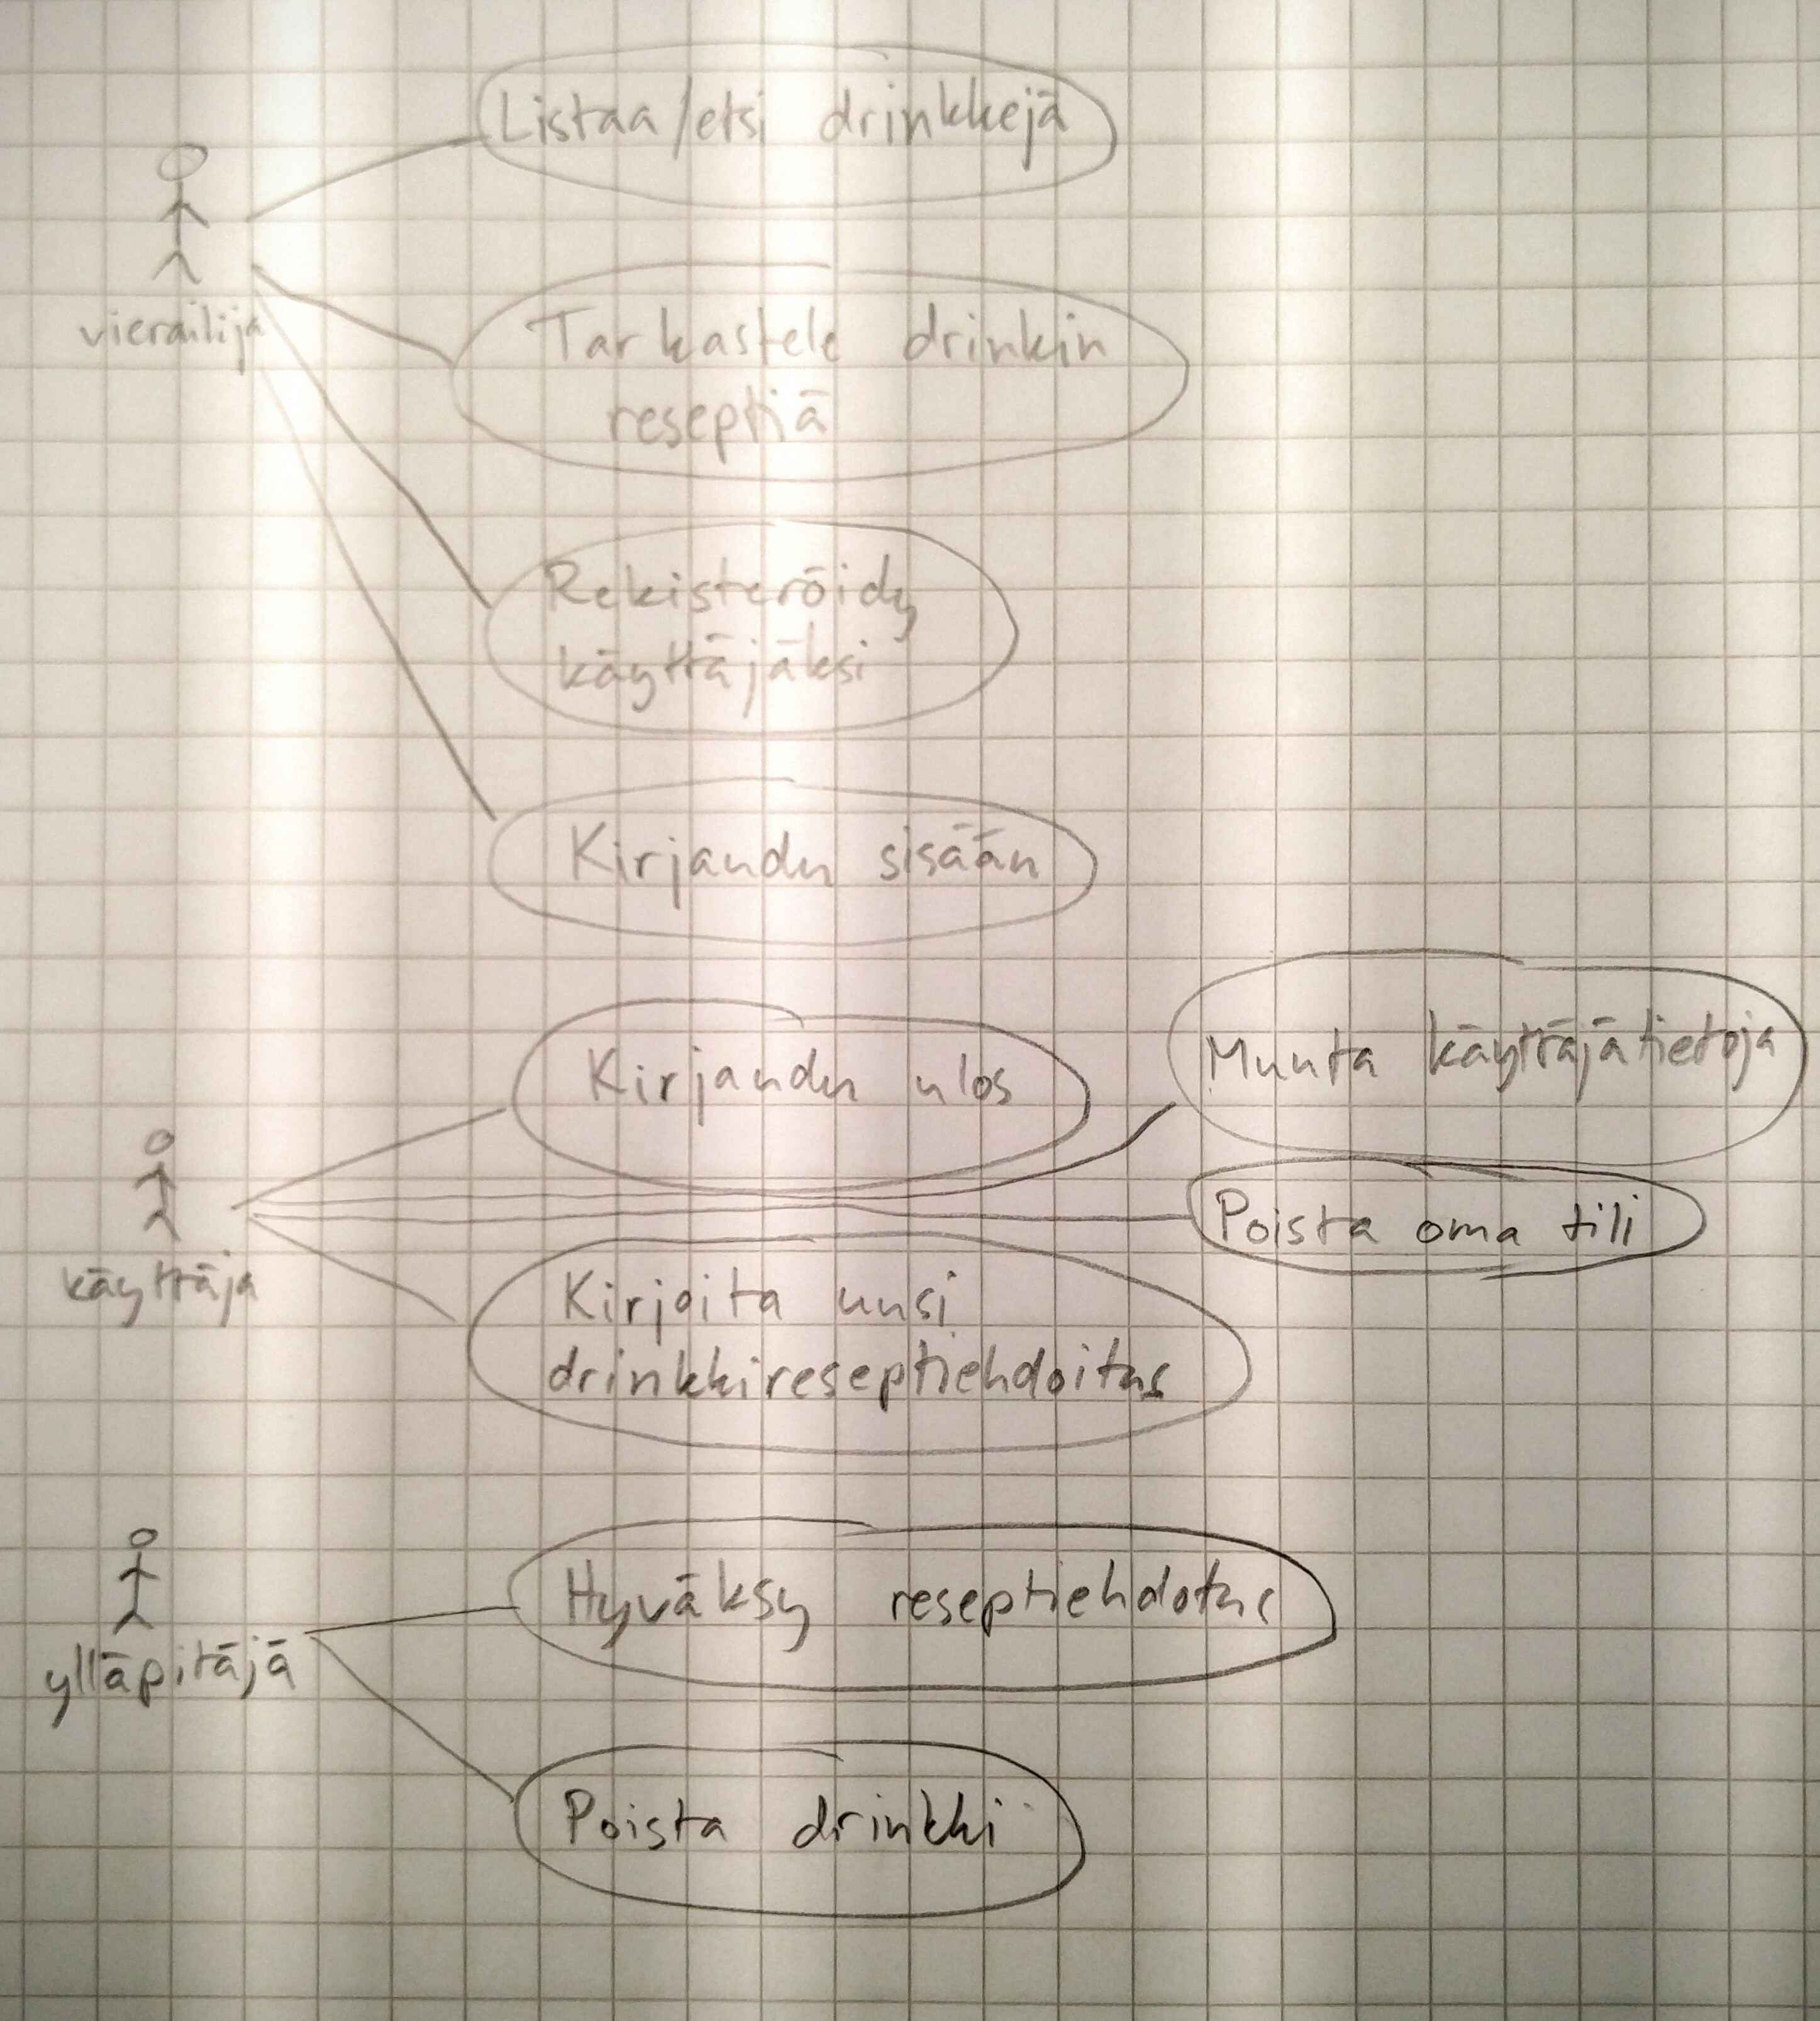
\includegraphics[width=\textwidth]{usecase-diagram}

\subsection{Käyttäjäryhmät}
\begin{description}
  \item[Vierailija] \hfill \\ Vierailijalla tarkoitetaan ketä tahansa joka vierailee sivulla.
  \item[Käyttäjä] \hfill \\ Käyttäjä on sivustolle rekisteröitynyt ja sisäänkirjautunut vierailija.
  \item[Ylläpitäjä] \hfill \\ Ylläpitäjä on käyttäjä, jonka tehtäviin ja oikeuksiin kuuluu reseptien hallinnointi.
\end{description}

\subsection{Käyttötapauskuvaukset}
\subsubsection{Vierailijan käyttötapaukset}
\begin{description}
  \item[Listaa drinkkejä] \hfill \\ Kun vierailija saapuu drinkkiarkiston etusivulle, hänelle näytetään lista uusimmista drinkeistä.
  \item[Etsi drinkkejä] \hfill \\ Drinkkiarkiston etusivulla on hakukenttä. Kun vierailija syöttää siihen hakusanan ja painaa hae-nappia (tai painaa enter), siirtyy hän hakutulossivulle joka näyttää hakua vastaavat drinkit.
  \item[Tarkastele drinkin reseptiä] \hfill \\ Kun vierailija klikkaa drinkkilistauksessa drinkin nimeä tai kuvaa, hän siirtyy reseptisivulle, jossa hän näkee drinkin tiedot tarkemmin, sisältäen drinkin ainesosat ja reseptin.
  \item[Muita käyttötapauksia] Rekisteröidy käyttäjäksi, Kirjaudu sisään
\end{description}

\subsubsection{Käyttäjän käyttötapaukset}
\begin{description}
  \item[Muuta käyttäjätietoja] \hfill \\ Kun käyttäjä on kirjautunut sisään, hänelle näytetään ''Oma profiili''-linkki. Sitä klikkaamalla käyttäjä pääsee sivulle jolla hänen tietonsa näkyvät muokattavissa tekstikentissä. Käyttäjä voi muokata tietojaan siitä, ja ''Tallenna''-nappia painamalla tallettaa muutokset.
  \item[Poista oma tili] \hfill \\ ''Oma profiili''-sivulla on nappi ''poista tili'', jota painamalla tili tuhotaan. Ennen tuhoamista sivu pyytää varmistuksen käyttäjältä.
  \item[Kirjoita uusi drinkkireseptiehdoitus] \hfill \\ Kun käyttäjä on kirjautunut sisään, hänelle näytetään ''Uusi drinkki''-linkki. Sitä klikkaamalla käyttäjä pääsee sivulle jossa on lomake uuden drinkkireseptin laatimiseen. Täytettyään lomakkeen käyttäjä painaa ''Ehdota drinkkiä''-nappia ja reseptiehdotus tallentuu tietokantaan.
  \item[Muita käyttötapauksia] Kirjaudu ulos
\end{description}
\subsubsection{Ylläpitäjän käyttötapaukset}
\begin{description}
  \item[Hyväksy reseptiehdoitus] \hfill \\ Kun ylläpitäjä on kirjautunut sisään, hänelle näytetään ''Reseptiehdotukset''-linkki. Sitä klikkaamalla ylläpitäjä pääsee sivulle joka listaa avoimet reseptiehdotukset. Hän näkee jokaisesta ehdotuksesta tarkat tiedot samalla sivulla. Jokaisen kohdalla on ''Hyväksy''- ja ''Hylkää''-napit, jotka tekevät vastaavat toimenpiteet reseptiehdotukselle.
  \item[Poista drinkki] \hfill \\ Kun ylläpitäjä tarkastelee drinkin reseptiä, hänelle näytetään ''Poista drinkki''-nappi. Sitä painamalla drinkki poistuu järjestelmästä.
\end{description}

\section{Järjestelmän tietosisältö}
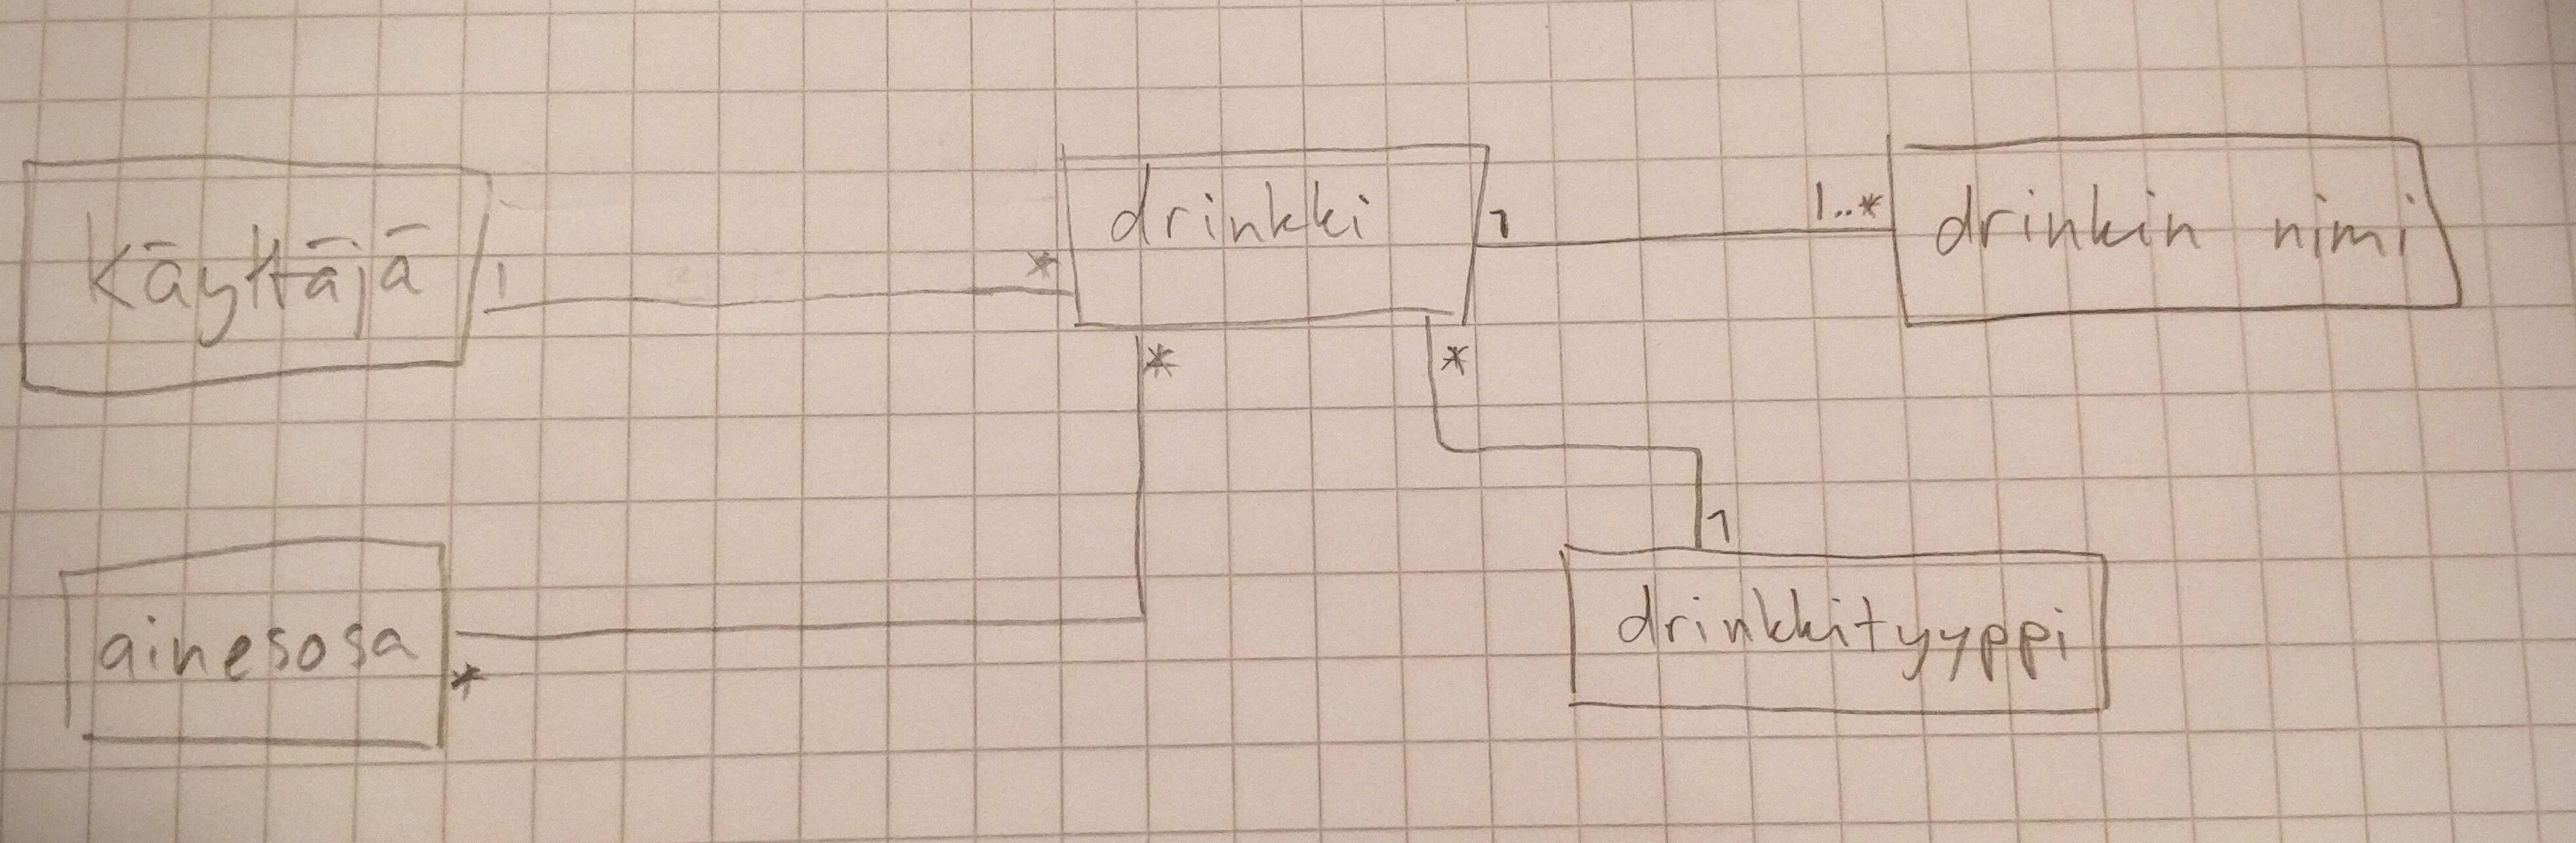
\includegraphics[width=\textwidth]{tietosisalto}

\section{Relaatiomalli}
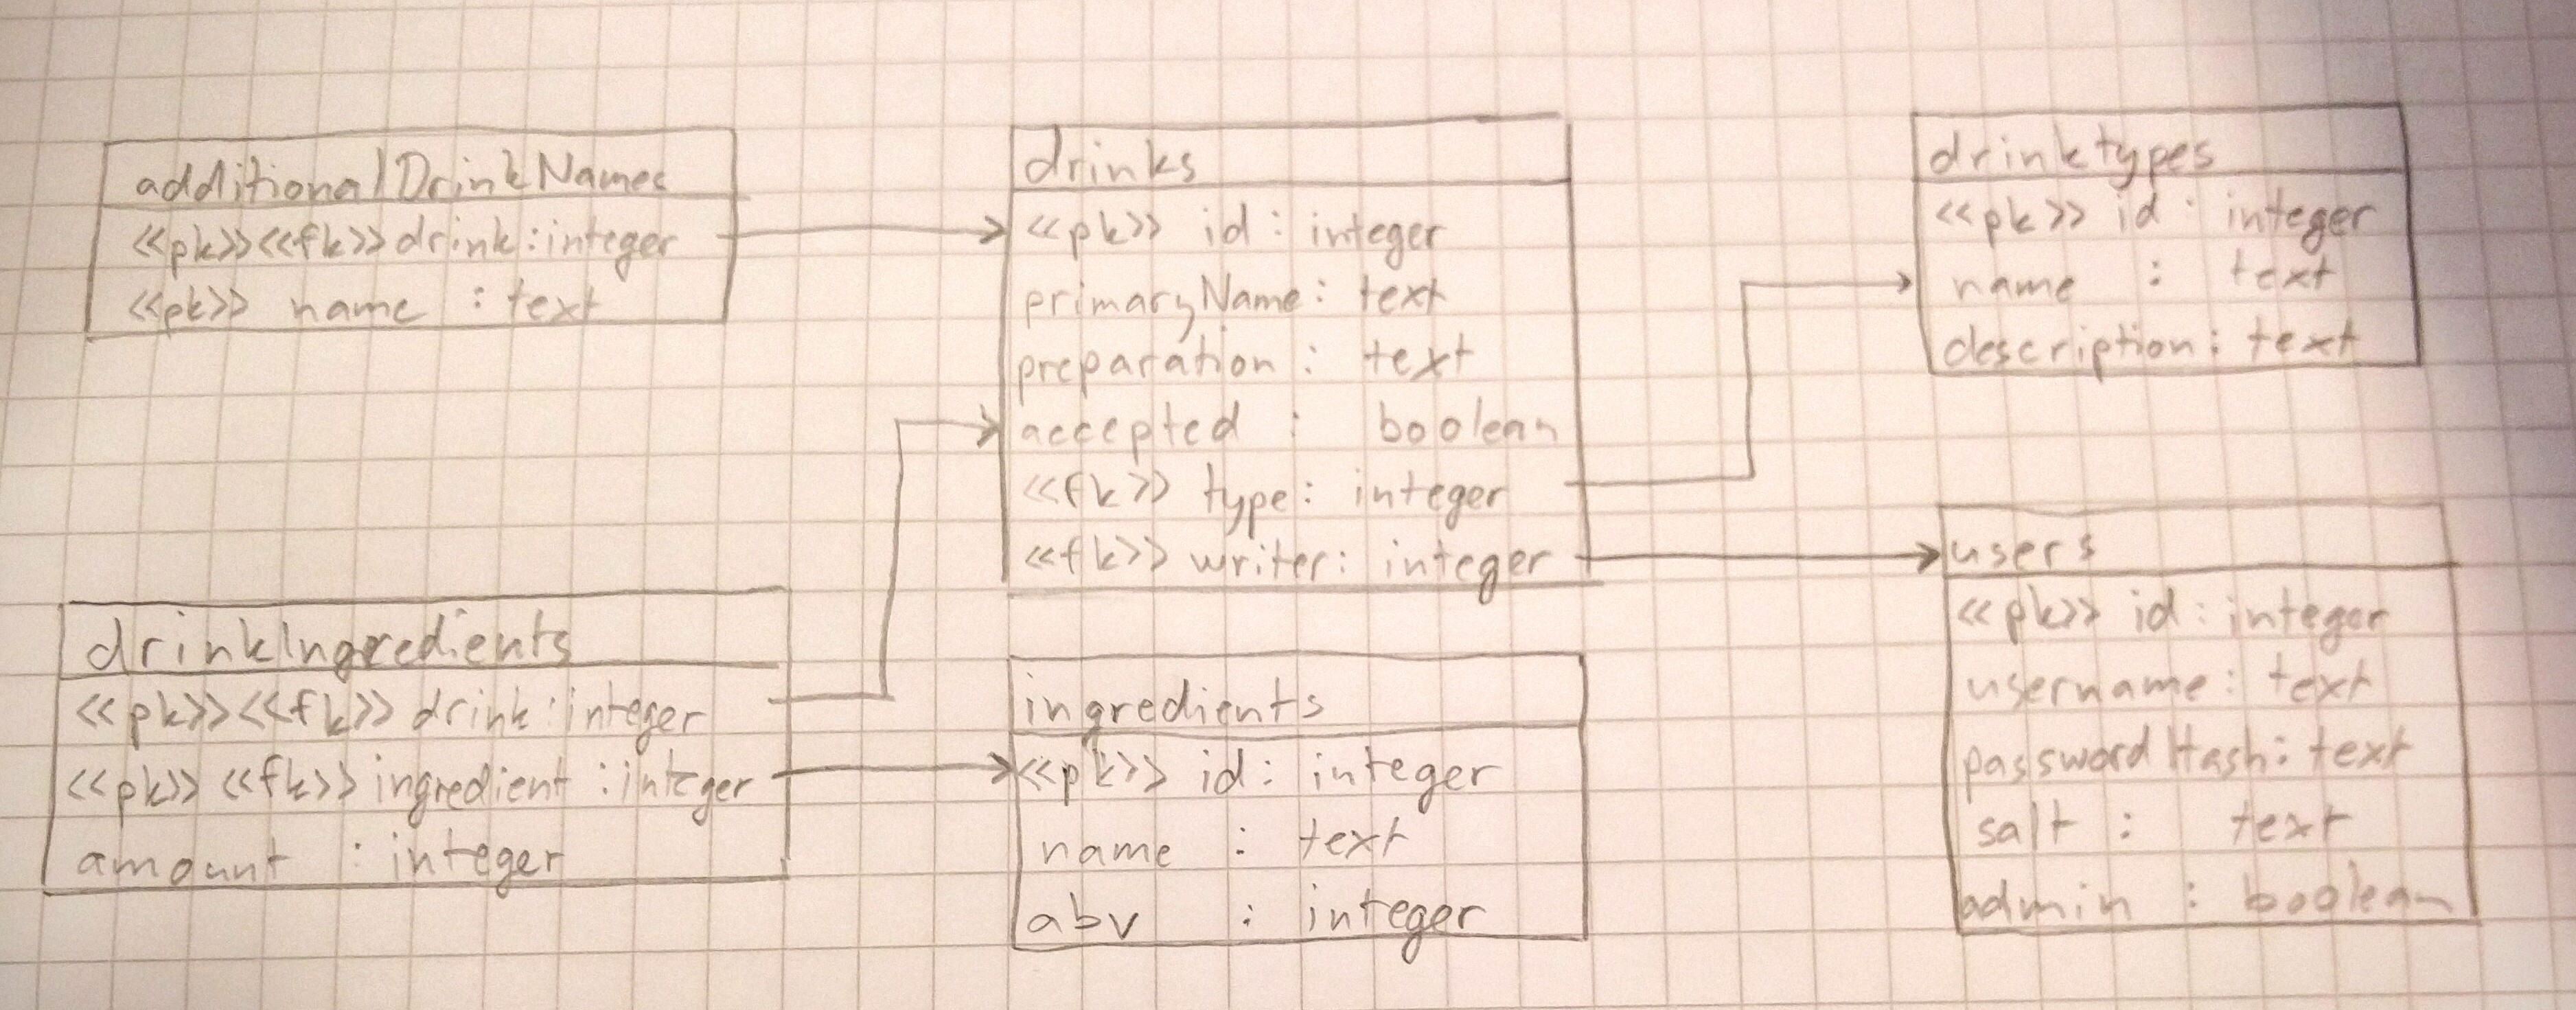
\includegraphics[width=\textwidth]{relation-diagram}

\section{Järjestelmän yleisrakenne}
TBD\ldots{}

\section{Käyttöliittymä ja järjestelmän komponentit}
TBD\ldots{}

\section{Asennustiedot}
TBD\ldots{}

\section{Käynnistys- ja käyttöohje}
Ohjelmiston demoinstanssi on osoitteessa \url{https://peaceful-scrubland-8625.herokuapp.com/}.

Sisään voi kirjautua yläpalkissa olevalla ''Kirjaudu sisään''-painikkeella. Käyttäjiä on kaksi: normaali käyttäjä user@example.com ja ylläpitäjä admin@example.com. Kummankin salasana on password.

Drinkkilistauksessa ja drinkkien sivuilla drinkin nimen vieressä on kuvakkeita. Kynäkuvake avaa muokkaussivun ja ruksi poistaa drinkin.

Kirjautuneet käyttäjät voivat lisätä drinkkejä, ja ylläpitäjät myös muokata ja poistaa niitä. Nappeja lisäystä, muokkausta ja poistoa varten ei näytetä, jos käyttäjällä ei ole oikeutta niihin.

\section{Testaus, tunnetut bugit ja jatkokehitys}
TBD\ldots{}

\section{Omat kokemukset}
TBD\ldots{}
\end{document}
